\documentclass[tikz,border=4pt]{standalone}
\usepackage[T1]{fontenc}
\usepackage{lmodern}
\usepackage{amsmath}
\usetikzlibrary{positioning,arrows.meta}
% Shared TikZ styles for the Methods workflow figures.
\usepackage{sansmath}
\renewcommand{\familydefault}{\sfdefault}
\sansmath
\newcommand{\step}[2]{\textbf{#1}\\[1pt]{\footnotesize #2}}
\tikzset{
  box/.style={draw, rounded corners=2pt, align=flush center, text width=10.4cm,
              inner sep=5pt, font=\small, line width=0.6pt},
  data/.style={box, draw=black!55, fill=black!6},
  proc/.style={box, draw=blue!55!black, fill=blue!7},
  filt/.style={box, draw=orange!75!black, fill=orange!10},
  result/.style={box, draw=green!45!black, fill=green!8},
  note/.style={align=left, font=\footnotesize\itshape, text=black!70},
  side/.style={box, text width=3.9cm, dashed, draw=black!55, fill=white},
  flow/.style={-{Stealth[length=2.2mm]}, line width=0.7pt, draw=black!65},
}


\begin{document}
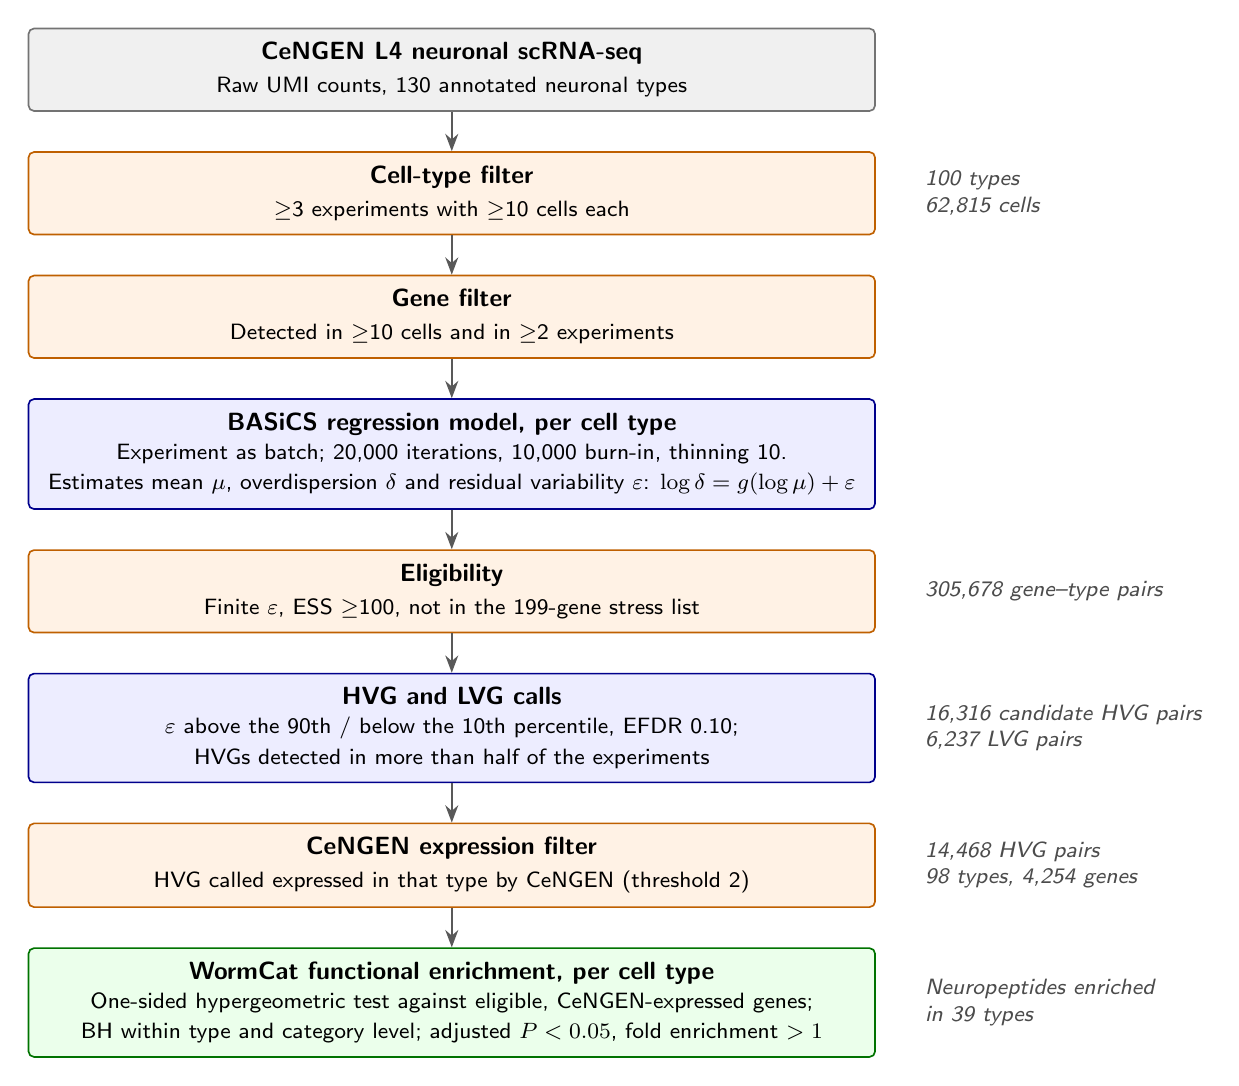
\begin{tikzpicture}[node distance=5mm]
\node[data]  (s1) {\step{CeNGEN L4 neuronal scRNA-seq}{Raw UMI counts, 130 annotated neuronal types}};
\node[filt, below=of s1] (s2) {\step{Cell-type filter}{$\ge$3 experiments with $\ge$10 cells each}};
\node[filt, below=of s2] (s3) {\step{Gene filter}{Detected in $\ge$10 cells and in $\ge$2 experiments}};
\node[proc, below=of s3] (s4) {\step{BASiCS regression model, per cell type}{Experiment as batch; 20,000 iterations, 10,000 burn-in, thinning 10.\\
  Estimates mean $\mu$, overdispersion $\delta$ and residual variability $\varepsilon$: $\log\delta = g(\log\mu)+\varepsilon$}};
\node[filt, below=of s4] (s5) {\step{Eligibility}{Finite $\varepsilon$, ESS $\ge$100, not in the 199-gene stress list}};
\node[proc, below=of s5] (s6) {\step{HVG and LVG calls}{$\varepsilon$ above the 90th / below the 10th percentile, EFDR 0.10;\\
  HVGs detected in more than half of the experiments}};
\node[filt, below=of s6] (s7) {\step{CeNGEN expression filter}{HVG called expressed in that type by CeNGEN (threshold 2)}};
\node[result,  below=of s7] (s8) {\step{WormCat functional enrichment, per cell type}{One-sided hypergeometric test against eligible, CeNGEN-expressed genes;\\
  BH within type and category level; adjusted $P<0.05$, fold enrichment $>1$}};

\foreach \a/\b in {s1/s2,s2/s3,s3/s4,s4/s5,s5/s6,s6/s7,s7/s8} \draw[flow] (\a) -- (\b);

\node[note, right=of s2] {100 types\\62,815 cells};
\node[note, right=of s5] {305,678 gene--type pairs};
\node[note, right=of s6] {16,316 candidate HVG pairs\\6,237 LVG pairs};
\node[note, right=of s7] {14,468 HVG pairs\\98 types, 4,254 genes};
\node[note, right=of s8] {Neuropeptides enriched\\in 39 types};
\end{tikzpicture}
\end{document}
